Eine Bungee-Springerin (\mJO) lässt sich von einer Brücke fallen. Das Seil ist \lSO\ lang und hat die Federkonstante \kSO. Bis Punkt (2) fällt sie frei, dann beginnt sich das Seil zu dehnen; im tiefsten Punkt (3) ist es um $s = \sSP{0}{3}$ gedehnt. Luftwiderstand und die Masse des Seils sind vernachlässigbar.
\begin{center}
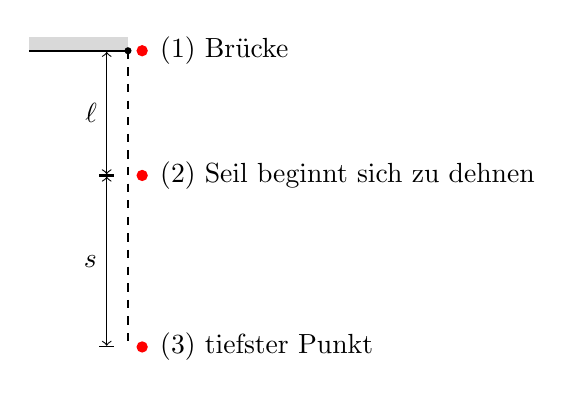
\begin{tikzpicture}[scale=0.09]
 \fill[gray!30] (-14,0) rectangle (0,2);
 \draw[thick] (-14,0) -- (0,0);
 \fill (0,0) circle (0.5);
 \draw[dashed] (0,0) -- (0,-41.8);
 \fill[red] (2,0) circle (0.8) node[right=3pt, black] {(1) Brücke};
 \fill[red] (2,-17.6) circle (0.8) node[right=3pt, black] {(2) Seil beginnt sich zu dehnen};
 \fill[red] (2,-41.8) circle (0.8) node[right=3pt, black] {(3) tiefster Punkt};
 \draw[|<->|] (-3,0) -- (-3,-17.6) node[midway, left] {$\ell$};
 \draw[|<->|] (-3,-17.6) -- (-3,-41.8) node[midway, left] {$s$};
\end{tikzpicture}
\end{center}
Ein Schüler hat die Energietabelle ausgefüllt. Nullniveau der Lageenergie ist der tiefste Punkt (3); gerechnet hat er mit \gO.
\begin{center}
\begin{tabular}{lccc}
 & $E_\mathrm{pot}$ & $E_\mathrm{kin}$ & $E_\mathrm{el}$ \\ \hline
 (1) Brücke & \EaP{3}{3} & \SI{0}{\joule} & \SI{0}{\joule} \\
 (2) Seil beginnt sich zu dehnen & \EbP{3}{3} & \EkbP{3}{3} & \SI{0}{\joule} \\
 (3) tiefster Punkt & \SI{0}{\joule} & \EkbP{3}{3} & \EcP{3}{3}
\end{tabular}
\end{center}

\begin{abcliste}
\abc
Ein Eintrag der Tabelle ist falsch. Welcher? \DuSie{Begründe}{Begründen Sie}.

\abc
Wie hätte der Schüler den Fehler mit einer Kontrolle der Gesamtenergie bemerken können?

\abc
Wie schnell ist die Springerin in (2)?
\end{abcliste}
